\chapter{Architecture}
Describe the different parts of your program suite in detail.
\\\\
kort inledning till kapitlet. vad har vi gjort i projektet?\\
trattigt namn, borde kanske ändras. ska innehålla typ metod - alltså vad har vi gjort?

\section{Finished work}
Running modules
What does your running code do? what is the output?

\subsection{Naive Bayes}

\subsection{K-Nearest Neighbour (KNN) algorithm}

\subsection{Support Vector Machine (SVM)}

\subsection{The Perceptron algorithm}
The Perceptron algorithm works as follows: 
The output, w, from the algorithm is a weight vector with the same size as y. If the classification for a x in the training set is equal to y, the weight is unchanged.
If y is 1 and the classification 0, then w is increased. If y is 0 and the classification 1, then w is decreased. \citep{perceptron_ai}
\begin{verbatim}
Let N = number of iterations through training set
Initialize the weight vector w to all zeros

Iterate N times through the training set:
    For each x, y in the training set:
        Let guess = classify(x) using our current w
        If y is not equal to guess:
            w := w + f(x, y) - f(x, guess)
Return w
\end{verbatim}
The Averaged Perceptron works in the same way except that it returns the average weight vector instead of the final.
This averaged vector is built incrementally by updating it while we build the usual weight vector. The pseudo code is the same as for the usual perceptron, except some lines which are shown below.
\begin{verbatim}
Initialize the average weight vector wa to all zeros and the counter c to 0.

If y is not equal to guess:
    w := w + f(x, y) - f(x, guess)
    average_weight := (N*T - c) / (N*T)
    wa := wa + average_weight * (f(x, y) - f(x, guess))
Increase the counter c
\end{verbatim}
In both of the Perceptron algorithms, the algorithm makes a number of iterations. The following plot was made to decide how many iterations that must be done to get a fair result. The algorithms uses input data of 2000 words (unigram) and 10-fold crossvalidaion. As seen in the plot, both the algorithms converge after around 15 iterations for both sentimental classification and text categorization.\\
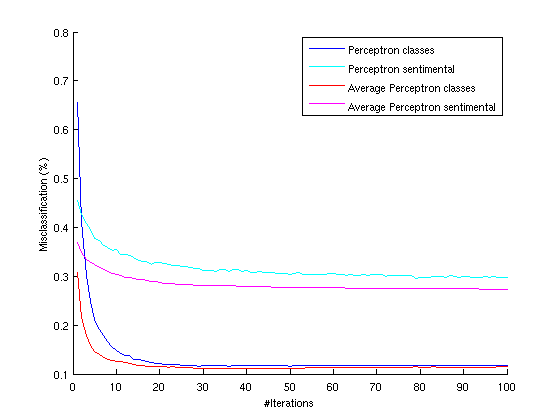
\includegraphics[scale = 0.8]{fig/perceptron_2000words_unigram_10foldcv_classes-high_sentimental-low.png}
